% !TeX root = ../geometry_main.tex
%=======================================================
%=======================================================
\chapter{Fibre bundles \&  tetrad formalism}
%=======================================================
%=============================================================


%-------------------------------------------------------
%=======================================================
\section{Fibre and principal bundles}\todotag{To be written}
%=======================================================
%------------------------------------------------------------


%---------------------------------------------------------------------
%=======================================================
\section{Tetrad formalism \& fiber-valued forms}\todotag{Polish all section} 
%=======================================================
%---------------------------------------------------------------------------
%

The tetrad formalism amounts to allowing arbitrary frames for the tangent $\{e_i(x)\}_i$ and cotangent  $\{\theta^i(x)\}_i$ bundles, not necessarily induced by a coordinate system.
It is the natural generalization to the framework needed for arbitrary fiber bundles $E_F\to M$.
The only typical requirement is the two frame be dual to each other i.e. $\theta^i (e_j) = \delta^i_j$.
In the literature, tetrads are also called \emph{vierbeins} (4-legs) in 4 dimensions or more generally \emph{vielbeins} (n-legs) in n dimensions.

To fix the notation, we reserve Greek letters $\mu,\nu,\rho\dots$ for coordinate indices and Latin letters $a,b,i,j,\dots$ for tetrad indices.
We use $\{\phi^a, f_a\}_a$ for tetrads of a generic fiber bundle $E_F\to M$, and $\{\theta^i,e_i\}_i$ for specific tetrads of the tangent bundle $TM\to M$.


\begin{mytheorem}[Avantages \& disadvantages of the tetrad formalism]
The main advantage of the tetrad formalism is that coefficients of tensors in arbitrary frames transform as scalars under coordinate transformations.
That is, their coordinates with respect to the tetrad bases do not change under change of coordinates, simply because we change the cohordinates $x^\mu\to \tilde{x}^\mu$ but the tetrad bases $\{e_a(x)\}_a$, $\{\theta^a(x)\}_a$ remain the same.
The main disadvantage is that expressions might get longer or more cumbersome, since we cannot use simplifications coming from coordinate bases e.g. the fact that $d (dx^\mu) = 0$ or $[\partial_\mu, \partial_\nu] = 0$.

In any case, this has several advtanges.
For example, we can choose a tetrad that is orthonormal wrt a given metric $g$ i.e. we have Minkowski (or Euclidean) metric at every point
\begin{equation}
    g = \eta_{ij} \theta^i \otimes \theta^j,\quad \eta_{ij}=\text{diag}(\pm1\dots \pm1)\,.
\end{equation}
This is particularly useful for spinors.
By definition, in any chosen frame, the $\gamma$ matrices are required to respect the Clifford algebra
\begin{equation}
    \{\gamma^\mu, \gamma^\nu\} = 2 g^{\mu\nu} \mathbb{I}.
\end{equation}
In such an orthonormal frame, this reduces to $\{\gamma^\mu, \gamma^\nu\} = 2 \eta^{\mu\nu} \mathbb{I}$, and we can thus take the $\gamma^\mu$ constantly equal to the usual Clifford algebra in flat space all over the manifold.
\end{mytheorem}


\begin{mytheorem}[Fiber valued differential forms ]
Fiber valued differential forms are just usual $p$-forms taking values in a fiber space $F$.
That is, given a fibre bundle $E_F\to M$ with fibre $F$, a fiber valued $p$-form is a \emph{section} of the product bundle
\begin{equation}
     E_F \otimes \Lambda^p (M) \to M.
\end{equation}
Given a local frame $\{f_a\}_a$ for the fiber bundle $E_F \to M$, any fiber valued $p$-form $\alpha \in \Lambda^p (M) \otimes E_F$ can be locally written as
\begin{equation}
    \alpha =  f_a \otimes \alpha^a,
\end{equation}
where $\alpha^a \in \Lambda^p (M)$ are ordinary differential $p$-forms.
\smallskip

We define a wedge product between any two fiber valued forms already at the level of linear spaces at each point $p\in M$
\begin{align}
    &E_F \otimes \Lambda^p (M)_{\mid p} \times E_G \otimes \Lambda^q (M)_{\mid p} \to (E_F \otimes E_G) \otimes \Lambda^{p+q} (M)_{\mid p} \quad \text{s.t.}\\[5pt]
    &\alpha,\,\beta \mapsto \alpha \wedge \beta := (f_a \otimes \alpha^a) \wedge (g_b \otimes \beta^b) 
    := (f_a \otimes g_b) \otimes (\alpha^a \wedge \beta^b) \in (E_F \otimes E_G) \otimes \Lambda^{p+q} (M).
\end{align}
The wedge prodcut naturally extends to sections of the fiber bundles i.e. fiber-valued differential forms.
\smallskip 

Notably, when $E_F = T^h_kM$ is the bundle of $(h,k)$-tensors we have tensor-valued differential forms, and this notion generalizes all the tensorial structures seen so far.
\begin{itemize}
    \item Ordinary differential $p$-form are just fiber valued $p$-form with trivial fiber $F = \mathbb{R}$.
    \item An $(h,k)$-tensor field is just a fiber valued $0$-form with fiber $F = T^h_k M$.
\end{itemize}
%
In fact, since $\Lambda^*(M)\subset T^*_*(M)$ the splitting in `differntial form part' and `tensor valued image' is somewhat arbitrary.
The most natural convention is to take all the antisymmetric part as the differential form part and the rest as the tensor valued image, as in the following examples.
\begin{itemize}
    \item The torsion $T_{\mu\nu}^{\, \rho}$, antisymmetric in the $\mu\nu$ indices, is a $(1,0)$-tensor valued 2-form i.e. a fiber valued 2-form with fiber $F = T^1_0 M$.
    \item The Riemann curvature $R_{\,\rho, \mu \nu}^{\sigma}$, antisymmetric in the $\mu\nu$ indices, is a $(1,1)$-tensor valued 2-form i.e. a fiber valued 2-form with fiber $F = T^1_1 M$.
\end{itemize}
\end{mytheorem}


\begin{mytheorem}[Exterior covariant derivative]
%
Given a fiber bundle $E_F \to M$ with fiber $F$ and a connection $\nabla$ on this bundle, we define the exterior covariant derivative $d_\nabla$ acting on fiber valued $p$-forms as the unique map
\begin{equation}
    d_\nabla: E_F \otimes \Lambda^\bullet (M)  \to E_F \otimes \Lambda^{\bullet +1} (M)
\end{equation}
thta is linear, satisfies the Leibniz rule 
\begin{equation}
    d_\nabla(\alpha \wedge \beta) = (d_\nabla \alpha) \wedge \beta + (-1)^p \alpha \wedge (d_\nabla \beta),\qquad \alpha \in E_F \otimes \Lambda^p (M),\, \beta \in E_G \otimes \Lambda^\bullet (M),
\end{equation}
and reduces to the usual covariant derivative $\nabla$ when acting on fiber valued $0$-forms and the usual exterior derivative $d$ when acting on ordinary differential forms i.e. fiber valued forms with trivial fiber $F = \mathbb{R}$.

\textbf{Beware  the exterior covariant derivative does not square to zero} in general, i.e. $d_\nabla^2 \neq 0$ due to the nontrivial connection 1-forms $\omega^a_b$.
\smallskip

Concretely, given a local frame $\{f_a\}_a$ for the fiber bundle $E_F \to M$, any fiber valued $p$-form $\alpha \in \Lambda^p (M) \otimes E_F$ can be locally written as $\alpha = f_a\otimes \alpha^a$.
The condition that $d_\nabla$ reduces to $\nabla$ on fiber valued $0$-forms and to the usual exterior derivative on forms with trivial fiber $F = \mathbb{R}$ implies that the exterior covariant derivative acts as
\begin{equation}
    d_\nabla \alpha = d_\nabla ( f_a\otimes \alpha^a)= \nabla f_a \wedge \alpha^a + f_a \otimes d \alpha^a  
    = f_a\otimes\left( \omega^a_{b} \wedge \alpha^b + d \alpha^a \right),
\end{equation}
where note that $f_a$ is a fiber valued $0$-form, and $\nabla f_a$ is a fiber valued $1$-form $T^1_0M\ni X \mapsto \nabla_X f_a \in F$, and $\omega^a_{b}$ are the connection 1-forms of the connection $\nabla$ in the chosen frame $\{f_a\}_a$.
\smallskip
\begin{proof}
The Leibniz rule is then obeyed since
\begin{align}
    d_\nabla(\alpha \wedge \beta) 
    &= \nabla (f_a\otimes g_b) \wedge (\alpha^a \wedge \beta^b) + (f_a\otimes g_b) \otimes d(\alpha^a \wedge \beta^b) \\
    &= \left( \nabla f_a \otimes g_b + f_a \otimes \nabla g_b \right) \wedge (\alpha^a \wedge \beta^b) +
    (f_a\otimes g_b) \otimes \left( d \alpha^a \wedge \beta^b + (-1)^p \alpha^a \wedge d \beta^b \right)
    \\
    &= f_a \otimes g_b \otimes \omega^a_{(F)\,c} \wedge \alpha^c \wedge \beta^b + f_a \otimes g_b \otimes \omega^b_{(G)\,d} \wedge \alpha^a \wedge \beta^d \\
    &\quad + f_a \otimes g_b \otimes d \alpha^a \wedge \beta^b + (-1)^p f_a \otimes g_b \otimes \alpha^a \wedge d \beta^b
    \\
    &= f_a\otimes\left( \omega^a_{(F)\,c} \wedge \alpha^c + d \alpha^a \right) \wedge (g_b \otimes \beta^b) + (-1)^p (f_a \otimes \alpha^a) \wedge \left( g_d \otimes \left( \omega^b_{(G)\,d} \wedge \beta^d + d \beta^b \right) \right)\\
    &=(d_\nabla \alpha) \wedge \beta + (-1)^p \alpha \wedge (d_\nabla \beta)\,.
\end{align}
\end{proof}
\end{mytheorem}


\begin{mytheorem}[Connection $\mathfrak{g}$-valued 1-form]
%
Given an affine connection $\nabla$ on a fibre bundle $E_F \to M$ with fiber $F$ and structure group $G$, define the $\mathfrak{g}$-valued connection 1-forms $\omega_F$ as the 1-form that in a given local frame $\{f_a\}_a$ for the fiber bundle $E_F \to M$ satisfy
\begin{equation}
     \nabla_X f_b=:\omega_F(X) f_b =: f_a\otimes \omega^a_{F\, b}(X)\,\quad \forall X \in \mathfrak{X}(M).
\end{equation}
The covariant derivative of a general section $\psi = \psi^a f_a$ is then given by the Leibniz rule 
\begin{equation}
    \nabla \psi = f_a \otimes (d\psi^a + \omega^a_{F\, b}\,\, \psi^b)\,.
\end{equation}
Under a change of local frame $\{\tilde{f}_a,\tilde{\phi}^a\}_a$ with $\tilde{f}_a= A_a^i f_i$ for some $A: U \subseteq M \to G$, the connection 1-form transforms as
\begin{equation}\label{eq:transformation_law_connection_1_form}
    \tilde{\omega}_a^b= (A^{-1})_j^b \,\, d A_a^j + (A^{-1})_j^b \,\, \omega^j_{i} \,\, A_a^i.
\end{equation}
This shows the connection 1-form does not transform as a tensor, due to the $A^{-1}\, dA$ piece, and is thus not \emph{tensor}-valued.
In fact, this is nothing else that the abstract tetrad form of the well-known transformation of Christoffel symbols under change of coordinates. (cf. connections on the tangent bundle below).

The connection 1-form is in fact a fiber-valued form with fiber the Lie algebra $\mathfrak{g}$ of the structure group $G$ of the frame bundle, e.g. $\mathfrak{gl}(n,\R)$ for general connections and $\mathfrak{so}(p,q)$ for orthonormal frames of metric connection with signature $(p,q)$.
Indeed the $\nabla$-parallel transport in $E_F\to M$ along a given curve $\gamma: [0,1] \to M$ yields linear isomorphisms (also metric-preserving if $\nabla$ is a metric connection)
\begin{align}
    P_\gamma(t): E_{F,\,\gamma(0)} &\to E_{F,\,\gamma(t)} \mid f \to P_\gamma(t)\,f\quad \text{for some curve }P_\gamma(t)\in G \subseteq GL(F),
\end{align}  
and the covariant derivative reurns the infinitesimal change,
\begin{align}
    P_\gamma(\epsilon) f = f + \epsilon \frac{d}{d t} \Big|_{t=0} P_\gamma(t) f + O(\epsilon^2) = f + \epsilon \nabla_{\dot{\gamma}(0)} f + O(\epsilon^2)\,.
\end{align}
This is simply a 1-parameter subgroup, which gives the commutative diagram of Lie groups and algebras
\[
    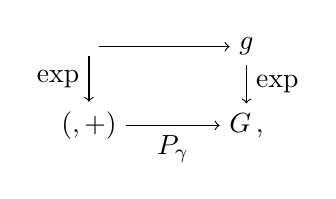
\begin{tikzpicture}[scale=1]
    \node (A) at (0,1) {$\R$};
    \node (B) at (2,1) {$\mathfrak{g}$};
    \node (C) at (0,0) {$(\R,+)$};
    \node (D) at (2,0) {$G\,,$};

    \draw[->] (A) -- node[above] {} (B);
    \draw[->] (A) -- node[left]  {$\exp$} (C);
    \draw[->] (B) -- node[right] {$\exp$} (D);
    \draw[->] (C) -- node[below] {$P_\gamma$} (D);
    \end{tikzpicture}
\]
Since the $\exp$ map is a local diffeomorphism, there exists $L\in\mathfrak{g}$ such that locally $P_\gamma(t) = \exp(L t)$ for $t\sim 0$.
Comparing the two expressions we thus confirm that
\begin{align}
    P_\gamma(\epsilon) f = \exp(\epsilon L)f = f + \epsilon L f + O(\epsilon^2) \quad \Rightarrow \quad \nabla_{\dot{\gamma}(0)} = \frac{\mathrm{d}P_\gamma}{\mathrm{d}t}_{\mid t=0}= L \in \mathfrak{g}.
\end{align}
%
In turn, we understand that the transformation law \eqref{eq:transformation_law_connection_1_form} of the connection 1-from is nothing else than the expected transformation at the Lie algebra level induced by the corresponding \emph{local} transformation of the represenation space $F$.
Indeed we can write at the level of abstract elements of $\mathfrak{g}$
\begin{align}
    \frac{\mathrm{d}P_\gamma}{\mathrm{d}t}f= \nabla_{\dot{\gamma}(t_0)} f 
    \quad \Rightarrow\quad P_\gamma(t) = \exp\left( \int_0^t \nabla_{\dot{\gamma}(\tau)} d\tau \right)
\end{align}
Now consider two local frames $\{f_i\}_i$ and $\{\tilde{f}_a = A_a^{i} f_i\}_a$ related by a local transformation $A: U \subseteq M \to G$, with connection 1-forms $\omega_{F}$ and $\tilde{\omega}_{F}$ respectively.
Representing the parallel transport isomorphism  $P_\gamma(t): {E_F}_{\gamma(0)} \longrightarrow {E_F}_{\gamma(t)}$ in both frames we find
\begin{align}
     P_\gamma(t)^j_i = \exp\left( \int_0^t \omega_{F}(\dot{\gamma}(\tau))\, d\tau \right)^j_i,
     \quad 
     &\tilde{P}_\gamma(t)^b_a = \exp\left( \int_0^t \tilde{\omega}_{F}(\dot{\gamma}(\tau))\, d\tau \right)^b_a = \big(A_{\gamma(t)}^{-1}\big)^b_j \, P_\gamma(t)^j_i \, \big(A_{\gamma(0)}\big)^i_a\\[5pt]
     \quad\Rightarrow\quad
    \tilde{\omega}_{F}(\dot{\gamma}(0))^b_a = \frac{d}{dt}\tilde{P}_\gamma(t)^b_a \Big|_{t=0} 
    &= \frac{d}{dt}_{|_{t=0}} \!\!\left( (A_{\gamma(t)}^{-1})^b_j \, P_\gamma(t)^j_i \, (A_{\gamma(0)})^i_a \right)\\[4pt]
    &= d(A^{-1})^b_j(\dot{\gamma}(0))\, (A_{\gamma(0)})_a^j + (A^{-1}_{\gamma(0)})^b_j \, \omega_{F}(\dot{\gamma}(0))^j_i \, (A_{\gamma(0)})^i_a.
\end{align}
This is precisely the transformation law \eqref{eq:transformation_law_connection_1_form} evaluated on the vector $\dot{\gamma}(0)\in T_{\gamma(0)}M$.\todotag{Check why sign of $dA$ differ}
%
\end{mytheorem}


\begin{mytheorem}[Connections on arbitrary fiber bundles induced from tangent bundle connection ]
The previous analysis suggests how to define arbitrary connections or how to extend a given connection to other fiber bundles.
Indeed, given an abstract $\mathfrak{g}$-valued 1-form $\omega\in \Gamma\left(\Lambda^1(M,\mathfrak{g})\right)$ and a fiber bundle $E_F\to M$ with structure group $G\curvearrowright F$ i.e. a representation $\rho: G \to GL(F)$, we can define a connection on $E_F\to M$ via
\begin{equation}
    \omega_F := \rho_*(\omega), \quad \text{that is}\quad \nabla_X f_b = f_a \otimes \omega^a_{F\, b}(X)\,,
\end{equation}
where $\rho_*: \mathfrak{g} \to \mathfrak{gl}(F)$ is the induced Lie algebra representation and $\{f_a\}$ is a local frame of $E_F\to M$.

The most common case is that we start with a connection $\nabla$ on the tangent bundle $TM\to M$.
Consider tetrads $\{e_i\}_i$ on the tangent bundle $T^1_0M\to M$ transforming under some (representation of a) structure group $G\subseteq GL(n,\R)$.
The connection form on the tangent bundle $\omega_{TM}$ must then take values in the representation of the Lie algebra $\mathfrak{g}\curvearrowright T^1_0M$ induced by the action of $G \curvearrowright T^1_0M$, with concrete matrix elements defined in the chosen tetrad $\{e_i\}_i$ as
\begin{align}
    \nabla_\cdot e_j &=: \omega_{TM}(\cdot) e_j =: e_i \otimes \omega^i_{\, j}(\cdot)\,.
\end{align}
It is automatic to extend the connection $\nabla$ on the cotangent bundle $T^0_1M$ via the ajoint representation of $\mathfrak{g}$, and to all tensor bundles $T^h_k M$ via the tensor product of (adjoint) representations.
Since the ajoint and tensor representations of $G$ are simply defined via parallel transport as
\begin{align}
    F^*\ni \varphi \mapsto \varphi\circ P_\gamma(t)^{-1}= \varphi_i\big(P_\gamma^{-1}\big)^i_j\quad  T^h_k F \ni T \mapsto P_\gamma(t) \circ T \circ P_\gamma(t)^{-1} = T^a_b \big(P_\gamma(t)\big)^c_a \big(P_\gamma^{-1}(t)\big)^b_d,
\end{align}
recalling that $P_\gamma(0)=\mathbb{I}$, $\frac{d(P_\gamma)^i_j}{dt}_{\mid t=0} = \omega^i_{\, j}$, and $\frac{d(P_\gamma^{-1})^i_j}{dt}_{\mid t=0} = - \omega^i_{\, j}$, we recover the familiar expressions for the connection 1-form (i.e. the associated Lie algebra representation) on adjoint and tensor representations
\begin{align}
    \nabla_\cdot \theta^i &=: \omega_{T^0_1M}(\cdot) \theta^i=: -\theta^j \otimes \omega^i_{\, j}(\cdot),\\
    \nabla_\cdot \big(e_a\otimes \theta^b\big) &=: \omega_{T^h_k M}(\cdot) \big(e_a\otimes \theta^b\big) =: e_c \otimes \theta^d \otimes \omega^{\binom{c}{d}}_{T^h_k M\, \binom{a}{b}}(\cdot) = e_c \otimes \theta^d \otimes \left( \omega^c_{\, a}(\cdot) \delta^b_d -\omega^b_{\, d}(\cdot) \delta^c_a\right).
\end{align}

Given an arbitrary fiber bundle $E_F\to M$ with the same structure group $G$ as the tangent bundle i.e. fiber $F$ transforming under some representation $G\curvearrowright F$ with corresponding Lie algebra representation $\mathfrak{g}\curvearrowright F$, we can also naturally induce a connection on $E_F\to M$.
Indeed, regardless of the specific representation, the connection 1-form on the tangent bundle can be seen as taking values in the \emph{abstract} Lie algebra
\begin{align}
    \omega: TM &\to \mathfrak{g} \,\, \mid T_pM \ni X \mapsto \omega(X) \in \mathfrak{g}.
\end{align}
We then simply define the connection 1-form $\omega_{F}$ on $E_F\to M$ as the 1-form taking values in the above representation of $\mathfrak{g}\curvearrowright F$.
In a given local frame $\{f_a\}_a$ for $E_F\to M$, the explicit matrix elements are defined as
\begin{align}
    \nabla_\cdot f_b &=: \omega_{F}(\cdot) f_b =: f_a \otimes \omega^a_{F\, b}(\cdot)\,.
\end{align}
By the Leibniz rule the covariant derivative of a general section $\psi = \psi^a f_a$ then reads
\begin{equation}
    \nabla \psi = f_a \otimes \big(d\psi^a + \omega_{F\, b}^a \, \psi^b\big)\,.
\end{equation}
In particular we remark that, as abstract elements of $\mathfrak{g}$, the connection 1-forms on $E_F\to M$ and on $TM\to M$ coincide i.e. $[\omega_{F}(\cdot)]\equiv [ \omega_{TM}(\cdot)] \equiv \omega(\cdot)\in \mathfrak{g}$.
\end{mytheorem}


\begin{mytheorem}[Metric compatibility in arbitrary fiber bundle]
%
Given a fiber bundle $E_F \to M$ with fiber $F$ and structure group $G$, endowed with a metric 
$g\in\Gamma(\otimes^2 E_F^*)$ and a connection $\nabla$ on $E_F$ with $\mathfrak{g}$-valued connection form $\omega$, we say that the connection is metric compatible if 
\begin{align}
    \nabla g \equiv 0\quad \text{i.e.}\quad d \left( g(s,t) \right) = g(\nabla s, t) + g(s, \nabla t)\quad \text{$\forall$ sections }s,t \in \Gamma(E_F).
\end{align}
In a tetrad $\{f_a\}_a$ for $E_F \to M$ with connection forms $\omega_{\,a}^{b}$ and metric $g_{ab} := g(f_a, f_b)$, the condition reads
\begin{equation}
    d g_{ab} = \omega_{\,a}^{c}\, g_{cb} + \omega_{\,b}^{c} \,g_{ac}.
\end{equation}
If the tetrad is orthonormal i.e. $g_{ab} \equiv \eta_{ab}= (\pm1\dots\pm1)$ constant with some signature $(p,q)$, the condition reduces to \emph{antisymmetry} of the connection 1-forms in this tetrad, upon lowering an index with the metric,
\begin{equation}
    0 = d(\eta_{ab})\quad \Rightarrow\quad \omega_{ab} = - \omega_{ba}\quad \text{ where }\quad \omega_{ab} := g_{ac} \, \omega^c_{~b}\,,
\end{equation}
confirming that in such tetrad the connection 1-form takes values in $\omega\in\mathfrak{so}(p,q)\subset \mathfrak{gl}(n)$.

\textbf{Antisymmetry} in the lowered indices is indeed the \textbf{hallmark of the Lie algebra $\mathfrak{so}(p,q)$.}
If $G\subseteq GL(T_pM) \equiv GL(n,\R)$ is the subgroup preserving the metric $g_p$ at point $p\in M$, for any curve $t\mapsto A(t)\sim\mathbb{I}+t\,\omega \in G\subseteq GL(T_pM)$
{\small
\begin{align}
    (g_p)_{\rho\sigma}A^\rho_\mu A^\sigma_\nu = (g_p)_{\mu\nu}
    &\Rightarrow 0 = \frac{d}{dt} \Big|_{t=0} \left( (g_p)_{\rho\sigma}A^\rho_\mu(t) A^\sigma_\nu(t) \right) = g_{\rho\sigma} \left( \frac{d}{dt} \Big|_{t=0} A^\rho_\mu(t) \right) \delta^\sigma_\nu + g_{\rho\sigma} \delta^\rho_\mu \left( \frac{d}{dt} \Big|_{t=0} A^\sigma_\nu(t) \right) \\
    &\Rightarrow g_{\rho\nu} \omega^\rho_\mu + g_{\mu\sigma} \omega^\sigma_\nu = 0.
\end{align}
}
This is indeed expected: a connection ultimately yields the infinitesimal change of a vector under parallel transport, and preserves angles and lengths by definition if it is metric compatible.
The \textbf{change of a vector} can thus only be an \textbf{infinitesimal `generalized rotation'} in the tangent space, i.e. an element of the Lie algebra of the orthogonal group of $g_p$, which is $SO(p,q)$ in a suitable basis.
\end{mytheorem}


\begin{mytheorem}[The example: connection on spinors]
%
Given a connection $\nabla$ on the tangent bundle $TM$ compatible with a metric of signature $(p,q)$,  we can naturally induce a connection on the spinor bundle $E_{\text{sp\tiny(p,q)}}\to M$ since its structure group--the spin group $\text{Spin}(p,q)$--is the double cover of $SO(p,q)$ and thus have the same Lie algebra $\mathfrak{so}(p,q)$, and we know how to get a representation $\mathfrak{so}(p,q) \to \mathfrak{gl}(\C^m)$ on the spinor space $\C^m$ in terms of gamma matrices satisfying the Clifford algebra.
\smallskip

If $\{e_{\mu}\}_\mu$ is an \emph{orthonormal} tetrad on $TM$ with $\mathfrak{so}(p,q)$-valued connection 1-forms $\omega^{\mu}_{{\text{\tiny TM}}\,\nu}$, and $\{s_a\}_a$ is a local tetrad of the spinor space with corresponding gamma matrices $\{\gamma^\mu\}_\mu$ satisfying the Clifford algebra $\{\gamma^\mu, \gamma^\nu\} = 2 \eta^{\mu\nu} \mathbb{I}$, we define the connection 1-forms on the spinor bundle $E_{\text{sp(\small p,q)}}$ by\footnote{Repeated indices are summed over, note that $S^{\mu\nu}=-S^{\nu\mu}$ and $\omega^{\text{\tiny TM}}_{\mu\nu}=-\omega^{\text{\tiny TM}}_{\nu\mu}$ cancels the $\tfrac12$ factor.}
\begin{align}
    \omega^{b}_{{\text{\tiny Sp}}\, a}&:= \tfrac12 \omega^{\text{\tiny TM}}_{\mu\nu} \big(S^{\mu\nu}\big)^b_{\,a} \quad \text{where}\quad \omega^{\text{\tiny TM}}_{\mu\nu}= g_{\rho\mu} \omega^\rho_{{\text{\tiny TM}}\, \nu}, \quad S^{\mu\nu} := \tfrac{1}{4} [\gamma^\mu, \gamma^\nu] = \tfrac12 \gamma^\mu\gamma^\nu\,.
\end{align}
The covariant derivative of a general spinor $\psi = s_a \psi^a$ is then
\begin{equation}
    \nabla \psi =  s_a d\psi^a + \psi^a \, \nabla s_a = s_b\otimes \left( d \psi^b + \omega^b_{\text{\tiny Sp}\, a} \, \psi^a \right)=
     s_b\otimes \left( d \psi^b + \tfrac{1}{8} \omega^{\text{\tiny TM}}_{\mu\nu}\, [\gamma^\mu, \gamma^\nu]^b_{\,a} \, \psi^a \right)\,.
\end{equation}
%
Finally consider another tetrad $\{\tilde{e}_i\}_i$ on $TM$, not necessarily orthonormal, related to the first one by $\tilde{e}_i= B_i^\mu e_\mu$.
The metric coefficients in such tetrad are then
\begin{align}
    \tilde{g}_{ij}:=g(\tilde{e}_i,\tilde{e}_j) = B_i^\mu B_j^\nu \eta^{\mu\nu}\,,\quad \tilde{g}^{ij} = (B^{-1})^i_\mu (B^{-1})^j_\nu \eta^{\mu\nu}.
\end{align}
If we take the same tetrad $\{s_a\}_a$ of the spinor space, then $\gamma$ matrices satisfying the Clifford algebra wrt the new metric $\tilde{g}_{ij}$ are given by
\begin{equation}
    \tilde{\gamma}^i = (B^{-1})^i_\mu \gamma^\mu \quad \Rightarrow \quad \{\tilde{\gamma}^i, \tilde{\gamma}^j\} = (B^{-1})^i_\mu (B^{-1})^j_\nu \{\gamma^\mu, \gamma^\nu\} = (B^{-1})^i_\mu (B^{-1})^j_\nu 2 \eta^{\mu\nu} = 2 \tilde{g}^{ij}\,.
\end{equation}
Inverting the relation $\gamma^\mu = B^\mu_i \tilde{\gamma}^i$, we can express the \textbf{connection 1-forms on the spinor bundle in terms of an arbitrary set of gamma matrices $\{\tilde{\gamma}^i\}_i$} as
\begin{align}
    \omega^{b}_{{\text{\tiny Sp}}\, a}&= \tfrac14 \omega^{\text{\tiny TM}}_{\mu\nu} \gamma^\mu\gamma^\nu 
    = \tfrac14 \omega^{\text{\tiny TM}}_{\mu\nu} B^\mu_i B^\nu_j \tilde{\gamma}^i \tilde{\gamma}^j\,.  
\end{align}
\end{mytheorem}


\begin{mytheorem}[Curvature 2-form ]
Given a connection $\nabla$ on a vector bundle $E_F\to M$ with structure group $G$, we define the $\mathfrak{g}$-valued curvature 2-form $\Omega$, often also denoted $R$ when we want to explicitate all the indices, as 
\begin{equation}
    R(X,Y) \equiv \Omega(X,Y) =\nabla_X \nabla_Y - \nabla_Y \nabla_X - \nabla_{[X,Y]}: E_{F\vert p} \to E_{F\vert p},\quad X,Y \in \mathfrak{X}(M)\,.
\end{equation}
This 2-form is indeed $\mathfrak{g}$ valued, since we already know the connection 1-form is.
Given a frame $\{\phi^a,f_a\}_a$, we define the $\R$-valued matrix curvature 2-forms $\Omega^b_{\, a}$ in this tetrad as
\begin{equation}
    R(X,Y) (f_a) = \Omega(X,Y) (f_a) = f_b \otimes \Omega^b_{\, a}(X,Y), \quad X,Y \in \mathfrak{X}(M)\,.
\end{equation}
The curvature form is indeed a `generalized rotation' in the fiber space, since it acts on a general section $S=S^a f_a$ as 
\begin{equation}
    R(X,Y) (S) = S^a R(X,Y) (f_a) = S^a f_b \otimes \Omega^b_{\, a}(X,Y).
\end{equation}
Given also a tetrad frame $\{\theta^\mu, e_\nu\}_\nu$ on $TM\to M$, we can explicitate all indices and write
\begin{align}
    \Omega_a^b= \tfrac12\underbrace{\Omega^b_a(e_\mu,e_\nu)}_{=:\R^b_{a,\,\mu\nu}}\theta^\mu \wedge \theta^\nu.
\end{align}
Finally under a change of tetrad $\{\tilde{f}_a,\tilde{\phi}^a\}_a$ on $E_F\to M$ with $\tilde{f}_a= A_a^i f_i$ for some $A: U \subseteq M \to G$, the curvature 2-form transforms \emph{tensorially} as it should
\begin{equation}
    \tilde{\Omega}_a^b= (A^{-1})_i^b \,\, \Omega^i_{j} \,\, A_a^j.
\end{equation}
The same happens chaning tetrads on the tangent bundle with $\tilde{e}_\mu = B_\mu^\rho e_\rho$ for some $B: U \subseteq M \to GL(n,\R)$ giving
\begin{equation}
    R^a_{b,\mu\nu}= B_\mu^\rho B_\nu^\sigma R^a_{b,\rho\sigma}.
\end{equation}
\end{mytheorem}


\begin{mytheorem}[Cartan structure equations]
%
Consider a connection $\nabla$ on a fiber bundle $E_F \to M$ with fiber $F$ and structure group $G$.
Given a tetrad frame $\{\phi^a,f_a\}_a$, consider the $(1,0)$ tensor valued 1-form $\phi :=  f_a \otimes \phi^a$.
The connection 1-form and curvature 2-form satisfy the Cartan structure equations, expressed concisely in terms of the exterior covariant derivative $d_\nabla$ as
\begin{align}
    T &:= d_\nabla \phi = f_a \otimes \left(d \phi^a + \omega^a_{\, b} \wedge \phi^b \right) 
    \quad \text{i.e.} \quad T^a = d \phi^a + \omega^a_{\, b} \wedge \phi^b,
    \\
    \Omega_{\, b} &= d_\nabla \omega_{\, b} = f_a \otimes \left(d \omega^a_{\, b} + \omega^a_{\,c} \wedge \omega^c_{\, b}\right) 
    \quad\text{i.e.} \quad \Omega^a_{\, b} = d \omega^a_{\, b} + \omega^a_{\, c} \wedge \omega^c_{\, b}.
\end{align}
The \textbf{Cartan equations are essentially definitions} of the torsion $T$ and curvature 2-form in terms of the connection 1-forms and the tetrad basis.
In fact, for \textbf{general fiber bundles} the first line is the \textbf{only available definition of torsion}, while it coincides with the usual torsion tensor in case $E_F = TM$ is the tangent bundle.
In particular, in absence of torsion $T=0$ the first Cartan structure equation reduces to
\begin{equation}
    d \phi^a + \omega^a_{\, b} \wedge \phi^b = 0.
\end{equation}
\end{mytheorem}
\vspace{-3mm}
\begin{proof}
From the definition of the exterior covariant derivative we have indeed
\begin{align}
    d_\nabla \phi &= d_\nabla (f_a \otimes \phi^a) = f_a \otimes d \phi^a  +  \nabla f_a \wedge \phi^a = f_a\otimes (d \phi^a + \omega^a_{\, b} \wedge \phi^b) ,
    \\
    d_\nabla \omega_{\, b} &= d_\nabla (f_a \otimes \omega^a_{\, b} ) = f_a\otimes d \omega^a_{\, b}  + \nabla f_a \wedge \omega^a_{\, b} = f_a\otimes (d \omega^a_{\, b} + \omega^a_{\, c} \wedge \omega^c_{\, b}).
\end{align}
For a general fibre bundle case, the first equation is just a definition of the torsion $T$ as the exterior covariant derivative of the tetrad 1-form $\phi$, and we need only to prove the second expression does indeed coincide with the usual curvature operator.
Using linearity of the 2-form, we prove it on a coordinate induced basis $\partial_\mu,\,\partial_\nu$ so that 
\begin{align}
    \Omega(\partial_\mu,\,\partial_\nu)(f_b)&:= \nabla_\mu \nabla_\nu f_b - \nabla_\nu \nabla_\mu f_b - \graycancel{\nabla_{[\partial_\mu,\,\partial_\nu]} f_b}
    \\
    &= \nabla_\mu \left( f_a \otimes \omega^a_{\, b}(\partial_\nu) \right) - \nabla_\nu \left( f_a \otimes \omega^a_{\, b}(\partial_\mu) \right)
    \\
    &= f_a \otimes \left( \partial_\mu \omega^a_{\, b}(\partial_\nu) + \omega^a_{\, c}(\partial_\mu) \, \omega^c_{\, b}(\partial_\nu) - \partial_\nu \omega^a_{\, b}(\partial_\mu) - \omega^a_{\, c}(\partial_\nu) \, \omega^c_{\, b}(\partial_\mu) \right)
    \\
    &\equiv f_a \otimes \left( d \omega^a_{\, b} + \omega^a_{\, c} \wedge \omega^c_{\, b} \right)(\partial_\mu,\,\partial_\nu) =: \left( d_\nabla \omega_{\, b} \right)(\partial_\mu,\,\partial_\nu).
\end{align}
%
\end{proof}


\begin{mytheorem}[Bianchi identities in the tetrad formalism]
%
The Bianchi identities in a tetrad $\{f_i,\,\phi^i\}_i$ are concisely expressed via the exterior covariant derivative $d_\nabla$ as
{\small\begin{align}
    &d_\nabla T:=d_\nabla(f_i\otimes T^i) = f_i\otimes\big( \Omega^i_{\, j} \wedge \phi^j\big)=:\Omega_j\wedge \phi^j\qquad \text{i.e.}\quad dT^i= \Omega^i_{\, j} \wedge \phi^j - \omega^i_{\, j} \wedge T^j,
    \\
    &d_\nabla\Omega_{\, j}:=d_\nabla\Big(f_i \otimes \Omega^i_{\, j}\Big) = f_i \otimes \Big(\omega_k^i\wedge \Omega^k_j + d \Omega_{\, j}^i\Big) = f_i \otimes \Omega^i_{\, k} \wedge \omega^k_{\, j}=:\Omega_k \wedge \omega^k_{\, j} \quad \text{i.e.}\quad d\Omega^i_j = \omega^i_k\wedge \Omega^k_j - \Omega^i_k \wedge \omega^k_{\, j}.
\end{align}}
Beware he exterior derivative of the $\R$-valued 2-forms $\Omega^i_{\, j}$ does NOT vanish, but rather it takes the form specified above.
The \textbf{Bianchi identities} essentially express \textbf{symmetry contraints} that follow \textbf{from the very definition} of torsion and curvature.
In particular, in absence of torsion $T=0$ the first Bianchi identity reduces to
\begin{equation}
    \Omega^i_{\, j} \wedge \phi^j = 0.
\end{equation}
\end{mytheorem}
\vspace{-3mm}
\begin{proof}
The first identity follows from direct computation of the exterior covariant derivative of the torsion 2-form and the second Cartan equation above, and is a good example of the fact that $d_\nabla^2\neq 0$ in general,
\begin{align}
    d_\nabla T &= d_\nabla (d_\nabla \phi) = d_\nabla \left[f_i\otimes \left(d \phi^i + \omega^i_{\, j} \wedge \phi^j \right)\right]
    \\
    &=
    f_i\otimes \left(\graycancel{d^2 \phi^i} + d\omega^i_{\, j} \wedge \phi^j \bluecancel{- \omega^i_{\, j} \wedge d\phi^j}  \right)
    + f_i \otimes \omega^i_k\wedge \left(\bluecancel{d \phi^k} + \omega^k_{\, j} \wedge \phi^j \right) 
    \\
    &=
    f_i \otimes \left( d\omega^i_{\, j} + \omega^i_{\, k} \wedge \omega^k_{\, j} \right) \wedge \phi^j
    \equiv \Omega_{\, j} \wedge \phi^j.
\end{align}
For the second equation, renaming dummy indices, expressing $\Omega^i_{\, j}$ in terms of $\omega$ and using it commutes under the wedge product since it is a 2-form, we have
\begin{align}
    d \Omega_{\,j}^i &= d \left( d \omega^i_{\, j} + \omega^i_{\, k} \wedge \omega^k_{\, j} \right) = \graycancel{d^2 \omega^i_{\, j}} + d\omega^i_{\, k} \wedge \omega^k_{\, j} - \omega^i_{\, k} \wedge d\omega^k_{\, j}
    \\
    &= \big(\Omega^i_k-\omega^i_\ell\wedge \omega^\ell_k\big)\wedge \omega^k_{\, j} - \omega^i_{\, k} \wedge \big(\Omega_j^k-\omega^k_\ell\wedge \omega^\ell_j\big)
    \\
    & = \Omega^i_k \wedge \omega^k_{\, j} - \omega^i_{\, \ell}\wedge \Omega^\ell_j
    \,\,\,\,\underbrace{-\omega^i_\ell\wedge \omega^\ell_k\wedge \omega^k_{\, j}
    + \omega^i_{\, k} \wedge \omega^k_\ell\wedge \omega^\ell_j}_{=0}
    = \Omega^i_k \wedge \omega^k_{\, j} - \omega^i_{\, \ell}\wedge \Omega^\ell_j.
\end{align}
The rest follows from the definition of the exterior covariant derivative.
\end{proof}





%===============================================================
\subsection{Tetrad formalism in the tangent bundle}
%===============================================================
%

\begin{mytheorem}[Structure constants of a tetrad frame]
%
Given a tetrad $\{\theta^i,e_i\}_i$ for the tangent bundle, the structure constants $C^i_{jk}$ are defined as the coefficients of the commutator expansion
\begin{equation}
    [e_j, e_k] = C^i_{jk} e_i \,\, \quad \text{antisymmetric in $j,k$}.
\end{equation}
By construction, the structure constants are antisymmetric in the two lower indices $C^i_{jk} = - C^i_{kj}$.
They measure the nonclosure of infinitesimal parallelograms constructed using the tetrad vector fields $\{e_i\}_i$.
%
They can be equivalently defined as the coefficients of the exterior derivative expansion
\begin{equation}
    d \theta^i = - \frac{1}{2} C^i_{jk} \theta^j \wedge \theta^k = - C^i_{j k} \,\, \theta^j \otimes \theta^k \quad \text{(sum over repeated indices)}.
\end{equation}
%
If two tetrads $\{e_i,\theta^i\}_i$ and $\{\tilde{e}_a, \tilde{\theta}^a\}_a$ are related by $\tilde{e}_a = A_a^{\, i} e_i$, by properties of the Lie brackets the structure constants transform as
\begin{equation}
    \tilde{C}^c_{ab} = (A^{-1})^c_k \left( C^k_{ij} A_a^{\, i} A_b^{\, j} + A_a^{\, i}\,\,\partial_{e_i} A_b^{\, k} - A_b^{\, j}\,\,\partial_{e_j} A_a^{\, k} \right).
\end{equation}
The \textbf{structure constants vanish} identically $C_{jk}^i \equiv 0$ if and only if the tetrad is \emph{holonomic} i.e. \textbf{induced by coordinates}  $\theta^\mu=dx^\mu,\,e_\nu=\frac{\partial}{\partial x^\nu}$, because of Frobenius theorem.
Then, if $e_i = B_i^\mu \partial_\mu$ for some coordinate system $\{x^\mu\}_\mu$, we can express the structure constants of another tetrad as
\begin{equation}\label{eq:structure_constants_from_coordinates}
    C_{ij}^k= (B^{-1})^k_\nu \left( B_i^\mu \partial_\mu B_j^\nu - B_j^\mu \partial_\mu B_i^\nu \right).
\end{equation}
%
Beware the structure constants make sense only for the tangent bundle $TM$ since only there we have a natural notion of commutator of vector fields, and in fact arbitrary fiber-valued forms are expressed as linear combinations of ordinary $\R$-valued forms times fiber basis elements.
\end{mytheorem}
\begin{proof}
Fix any coordinate system $\{x^\mu\}_\mu$ and let $\theta^i = \theta^i_\mu dx^\mu$, $e_j = e_j^\nu \partial_\nu$.
By duality of the tetrad we have
\begin{align}
    0= \partial_\mu \delta^i_j &= \partial_\mu \big(\theta^i (e_j) \big) = \partial_\mu\big(\theta^i_\nu e_j^\nu \big) = (\partial_\mu \theta^i_\nu) e_j^\nu + \theta^i_\nu (\partial_\mu e_j^\nu)
    \quad \Rightarrow\quad (\partial_\mu \theta^i_\nu) e_j^\nu =- \theta^i_\nu (\partial_\mu e_j^\nu)\,.
\end{align}
By definition of exterior derivative we have
\begin{align}
    d \theta^i &= (\partial_\mu \theta^i_\nu) dx^\mu \wedge dx^\nu = \partial_\mu \theta^i_\nu \Big(dx^\mu\otimes dx^\nu- dx^\nu \otimes dx^\mu \Big)\,.
\end{align}
Evaluating on the tetrad and using the previous relation we get
\begin{align}
    d\theta^i (e_j, e_k) 
    = \partial_\mu \theta^i_\nu \Big( e_j^\mu e_k^\nu - e_j^\nu e_k^\mu \Big) 
    = - \theta^i_\nu \Big( (\partial_\mu e_j^\nu) e_k^\mu - (\partial_\mu e_k^\nu) e_j^\mu \Big) 
     =: - \theta^i \big( [e_j, e_k]\big) = - C^i_{jk}\,.
\end{align}
That is to say
\begin{align}
    d\theta^i = - \frac{1}{2} C^i_{jk} \theta^j \wedge \theta^k\, \Leftrightarrow [e_j, e_k] = C^i_{jk} e_i\,.
\end{align}
Finally the fact that $C_{ij}^k \equiv 0$ if and only if $e_\mu\equiv \partial_\mu$ for some coordinate system $\{x^\mu\}_\mu$ follows from Frobenius theorem.
%
\end{proof}


\begin{mytheorem}[Christoffel symbols in a tetrad frame of the tangent bundle]
Given a tetrad $\{\theta^i,\, e_i\}_i$ on the tangent bundle $TM\to M$ with affine connection \(\nabla\), define the Christoffel symbols \(\Gamma^i_{jk}\) by
\begin{equation}
    \nabla_{e_j} e_k =: \Gamma^i_{jk} e_i\,,\qquad\text{that is}\qquad \omega^i_{\, k}(\cdot) = \Gamma^i_{ jk}\,\, \theta^j(\cdot).
\end{equation}
Under a change of tetrad \(\{\tilde{\theta}^a,\, \tilde{e}_a\}_a\) related to the previous one by \(\tilde{e}_a = A_a^{\, j} e_j\), the Christoffel symbols transform as
\begin{equation}
    \tilde{\Gamma}^c_{ab} = (A^{-1})^c_k \left( \Gamma^k_{ij} A_a^{\, i} A_b^{\, j} + A_a^{\, i}\,\,\partial_{e_i} A_b^{\, k}  \right).
\end{equation}
%
For a metric connection $\nabla g\equiv 0$ with arbitrary torsion $T$, the \textbf{Koszul formula} is
\begin{align}\label{eq:koszul_formula}
\begin{aligned}
    2\,g(\nabla_X Y, Z) ={}& X\!\left(g(Y,Z)\right) + Y\!\left(g(Z,X)\right) - Z\!\left(g(X,Y)\right)\\
    &\, + g([X,Y],Z) - g([Y,Z],X) - g([X,Z],Y) \\
    & \,+ g\!\left(T(X,Y),Z\right) - g\!\left(T(Y,Z),X\right) - g\!\left(T(X,Z),Y\right).
\end{aligned}
\end{align}
We then express the Christoffel symbols in terms of metric $g_{ij} := g(e_i, e_j)$, structure constants \(C^i_{\, jk}:=\theta^k([e_i,e_j])\) and torsion components \(T^i_{\, jk}:=\theta^i(T(e_j,e_k))\) in a given tetrad as
\begin{align}\label{eq:koszul_formula_cohordinates}
\begin{aligned}
    \Gamma_{ij}^k=&\tfrac{1}{2} g^{k\ell} \Big( \partial_{e_i}\,g_{j \ell} + \partial_{e_j}\,g_{i \ell} - \partial_{e_\ell}\,g_{i j}\Big)\\
    & + \tfrac{1}{2} g^{k\ell} \Big( g_{m \ell} C^m_{ij}  - g_{m i} C^m_{j \ell}  - g_{m j} C^m_{i \ell}\Big) \\
    & +\tfrac{1}{2} g^{k\ell} \Big( g_{m \ell} T^m_{ij} -g_{m i} T^m_{j \ell} - g_{m j} T^m_{i \ell}  \Big).
\end{aligned}
\end{align}
If $C_{ij}^k\equiv 0$ we recover usual expression for Christoffel symbols in a coordinate basis\footnote{In fact we have $C_{ij}^k\equiv 0$ iff there exist some coordinates $x^\mu$ s.t. $e_\mu=\partial_\mu$ by Frobenius theorem.}, split into symmetric and antisymmetric part in the lower indices 
\begin{equation}
    \Gamma_{(ij)}^k=\tfrac{1}{2} g^{k\ell} \Big( \partial_{e_i}\,g_{j \ell} + \partial_{e_j}\,g_{i \ell} - \partial_{e_\ell}\,g_{i j}\Big) - \tfrac{1}{2} g^{k\ell} \Big( g_{m i} T^m_{j \ell} + g_{m j} T^m_{i \ell}  \Big)\,,
    \quad \Gamma_{[ij]}^k = \tfrac{1}{2} T^k_{ij}\,.
\end{equation}
In the absence of torsion the second line vanishes, but $\Gamma_{ij}^k$ is not yet symmetric in general in the lower indices due to the possibly nonzero structure constants $C_{ij}^k=[e_i,e_j]^k$.

Finally in an orthonormal frame $g_{ij}:=g(e_i,e_j) = \eta_{ij}$ and the first line $\propto \, \partial g$ vanishes.
If $e_i=B_i^\mu\partial_\mu$ for some coordinate system $\{x^\mu\}_\mu$, we can express the Christoffel symbols as
\begin{align}
\begin{aligned}
    \Gamma_{ij}^k=&\tfrac{1}{2} \eta^{k\ell} \Big( \eta_{m \ell} C^m_{ij}  - \eta_{m i} C^m_{j \ell} - \eta_{m j} C^m_{i \ell}\Big) \\
    & +\tfrac{1}{2} \eta^{k\ell} \Big( \eta_{m \ell} T^m_{ij} -\eta_{m i} T^m_{j \ell} - \eta_{m j} T^m_{i \ell}  \Big),\quad \text{where}\quad C_{ij}^k= (B^{-1})^k_\nu \left( B_i^\mu \partial_\mu B_j^\nu - B_j^\mu \partial_\mu B_i^\nu \right).
\end{aligned}
\end{align}
\end{mytheorem}
\begin{proof}
By metric compatibility $\nabla g=0$, that is $0=X(g(Y,Z)) - g(\nabla_X Y,Z) - g(Y, \nabla_X Z)$.
By definition of torsion $\nabla_X Y = \nabla_Y X + [X,Y] + T(X,Y)$.
Permuting the vector fields $X,Y,Z$ cyclically and using these two identities we get the Koszul formula.
Setting \(X=e_j,\, Y=e_k,\, Z=e_i\), using the definition of the Christoffel symbols and structure constants, and then raising indices with the metric inverse gives the final expression.
\end{proof}


\begin{mytheorem}[Torsion 2-form in a tetrad frame on the tangent bundle]
%
In the case of the tangent bundle we can equivalently define the torsion $T_0^1$-valued 2-form as 
\begin{equation}
    T(X,Y) = \nabla_X Y - \nabla_Y X - [X,Y],\quad X,Y \in \mathfrak{X}(M).
\end{equation}
Beware this naive definition makes sense only for the tangent bundle since we need the notion of commutator of vector fields $[X,Y]$.
Indeed torsion measures the nonclosure of the parallelogram obtained by following the flow of the first vector field, then the flow of the parallel transport of the second vector field along the first, and then viceversa, an operation which is only defined on the manifold.

Given a tetrad frame \(\{\theta^i,\, e_i\}_i\) on the tangent bundle \(TM\to M\) with structure constants \(C^i_{jk}\) and a connection \(\nabla\) with Christoffel symbols \(\Gamma^i_{jk}\), the torsion 2-forms in this tetrad read
\begin{equation}
    T^i = \tfrac{1}{2} T^i_{jk} \,\, \theta^j \wedge \theta^k,
    \qquad \text{where}\qquad
    T^i_{jk} = \Gamma^i_{jk} - \Gamma^i_{kj} - C^i_{jk}.
\end{equation}
Beware torsion is not always antisymmetric in the lower indices, because of the nontrivial structure constants contribution.
In a coordinate induced frame $C_{ij}^k\equiv0$, and we recover the usual (antisymmetric) expression for the torsion components.
%
\end{mytheorem}



\begin{mytheorem}[Riemann curvature tensor in a tetrad frame on the tangent bundle]
%
Given a tetrad frame \(\{\theta^i,\, e_i\}_i\) with structure constants \(C^i_{jk}\) and a connection $\nabla$ on the tangent bundle $TM$ with Christoffel symbols \(\Gamma^i_{jk}\), we can express the curvature 2-forms as
\begin{equation}
    \Omega^\ell_{\, k} = \tfrac{1}{2} R^\ell_{k,\,ij} \,\, \theta^i \wedge \theta^j.
\end{equation}
The components of the Riemann tensor in this tetrad can be further explicitated as
\begin{equation}
    R^\ell_{k,\,ij} = \partial_{e_i} \Gamma^\ell_{j k} - \partial_{e_j} \Gamma^\ell_{i k} + \Gamma^\ell_{i m} \Gamma^m_{j k} - \Gamma^\ell_{j m} \Gamma^m_{i k} - C^m_{ij} \Gamma^\ell_{m k}.
\end{equation}
In a coordinate induced frame $C_{ij}^m\equiv0$ and we recover the usual expression for the Riemann tensor components.

More generally, we can plug in formula \eqref{eq:koszul_formula_cohordinates} for the Christoffel symbols to express the Riemann tensor purely in terms of metric $g_{ij}$, structure constants $C_{ij}^k$ and the \emph{arbitrary} torsion $T_{ij}^k$.
%
If we consider an orthonormal tetrad $e_a = B_a^\mu \partial_\mu$ related to some coordinate system $x^\mu$, we can also express everything in terms of the torsion and the matrix $B$ and its derivatives, using formula \eqref{eq:structure_constants_from_coordinates} for the structure constants.
\end{mytheorem}



\begin{mytheorem}[Cartan structure equations]
%
Consider a connection $\nabla$ on the tangent bundle $TM \to M$.
Given a tetrad frame $\{\theta^i,e_j\}_i$, consider the $(1,0)$ tensor valued 1-form $\theta :=  e_i \otimes \theta^i$.
The connection 1-form, and the torsion and curvature 2-forms satisfy the Cartan structure equations, expressed concisely in terms of the exterior covariant derivative $d_\nabla$ as
\begin{align}
    T &= d_\nabla \theta := d_\nabla (e_a\otimes \theta^a)= e_a \otimes \left(d \theta^a + \omega^a_{\, b} \wedge \theta^b \right) 
    \quad \text{i.e.} \quad T^a = d \theta^a + \omega^a_{\, b} \wedge \theta^b,
    \\
    \Omega_{\, b} &= d_\nabla \omega_{\, b}:=d_\nabla (e_a \otimes \omega^a_{\, b}) = e_a \otimes \left(d \omega^a_{\, b} + \omega^a_{\,c} \wedge \omega^c_{\, b}\right) 
    \quad\text{i.e.} \quad \Omega^a_{\, b} = d \omega^a_{\, b} + \omega^a_{\, c} \wedge \omega^c_{\, b}.
\end{align}
The \textbf{Cartan equations are essentially definitions} of the torsion and curvature 2-forms in terms of the connection 1-forms and the tetrad basis.
In the case of the tangent bundle, the first line does indeed coincides with the \textbf{usual definition of torsion} tensor.
In particular, in \textbf{absence of torsion $T=0$ the first Cartan equation} reduces to
\begin{equation}
    d \theta^a + \omega^a_{\, b} \wedge \theta^b = 0.
\end{equation}
\end{mytheorem}
\vspace{-4mm}
\begin{proof}
The second equalities just follow from the definition of the exterior covariant derivative and are already shown in the case of general fibre bundles above.
We need to show the expressions coincide with the old notions of torsion and curvature tensors.
Since the identity are tensorial, we can prove them by direct computation using a coordinate frame $\{\theta^\nu=dx^\nu,\, e_\nu=\partial_{x^\nu}\}_\nu$, the known expressions $T\sim \Gamma - \Gamma^T$ and $R\sim \partial \Gamma + \Gamma \Gamma$ for the torsion and Riemann tensor, and the relations
\begin{align}
    \theta^\rho = dx^\rho,\quad d\theta^\rho = 0,\quad
    \omega^\rho_{\, \nu} = \Gamma^\rho_{\mu \nu} dx^\mu,
    \quad
    d \omega^\rho_{\, \nu} = \partial_\sigma \Gamma^\rho_{\mu \nu} dx^\sigma \wedge dx^\mu,
    \quad
    \omega^\rho_{\, \sigma} \wedge \omega^\sigma_{\, \nu} = \Gamma^\rho_{\mu \sigma} \Gamma^\sigma_{\lambda \nu} dx^\mu \wedge dx^\lambda.
\end{align}
%
\end{proof}



\begin{mytheorem}[Bianchi identities on the tangent bundle \& recovering coordinate formalism]
%
The Bianchi identities on the tangent bundle are unchanged from a general fiber bundle and so is the proof.
In a tetrad $\{e_a,\theta^a\}_a$ of $TM\to M$ they read
{\small
\begin{align}
    &d_\nabla T :=d_\nabla\big(e_a\otimes T^a\big)= e_a\otimes \big(\Omega^a_b \wedge \theta^b\big) = \Omega_{\, b} \wedge \theta^b\qquad \text{i.e.}\quad dT^a = -\omega_b^a\wedge T^b +\Omega^a_{\, b} \wedge \theta^b,
    \\
    &d_\nabla \Omega_{\, b} :=d_\nabla (e_a \otimes \Omega^a_{\, b})\!=\! e_a \!\otimes\! \Big(\omega_c^a\wedge \Omega^c_b + d \Omega_{\, b}^a\Big) = e_a \!\otimes\! \Big(\Omega^a_{\, c} \wedge \omega^c_{\, b}\Big) =: \Omega_c \wedge \omega^c_{\, b} \,\, \,\text{i.e.}\,\,\, d\Omega^a_b = -\omega^a_c\wedge \Omega^c_b + \Omega^a_c \wedge \omega^c_{\, b}.
\end{align}}
Beware the exterior derivative of the $\R$-valued 2-forms $\Omega^i_{\, j}$ does NOT vanish, but rather takes the form specified above.
The \textbf{Bianchi identities} essentially express \textbf{symmetry contraints} that follow \textbf{from the very definition} of torsion and curvature.
\end{mytheorem}


\begin{mytheorem}[Cartan \& Bianchi equations in the absence of torsion]
In the absence of torsion $T\equiv 0$, the Cartan equations and Bianchi equations become respectively
\begin{align}\label{eq:cartan_bianchi_no_torsion}
    \begin{cases}
    d \theta^a + \omega^a_{\, b} \wedge \theta^b = 0,
    \\[4pt]
    d \omega^a_{\, b} + \omega^a_{\, c} \wedge \omega^c_{\, b} = \Omega^a_{\, b},
    \end{cases}
    \qquad\qquad
    \begin{cases}
    \Omega^a_{\, b} \wedge \theta^b = 0,
    \\[4pt]
    d \Omega^a_{\, b} = \Omega^a_{\, c} \wedge \omega^c_{\, b} - \omega^a_c\wedge \Omega^c_b.
    \end{cases}
\end{align}
Taking the exterior derivative of the first and using the second Cartan equation we get the first Bianchi identity, while taking the exterior derivative of the second Cartan equation we get the second Bianchi identity.
Hence \textbf{Cartan equations imply the Bianchi identities in the absence of torsion.}
\end{mytheorem}


\begin{mytheorem}[Recasting information from the metric into the tetrad]
%
Let us now assume $\nabla$ is the Levi-Civita connection of a Lorentzian metric $g$ on $M$ with vanishing torsion $T\equiv 0$.
The Cartan and Bianchi equations in the absence of torsion reduce to \eqref{eq:cartan_bianchi_no_torsion}.
If we consider \emph{orthonormal} tetrads $e_a$ the metric is trivial $g_{ab}\equiv \eta_{ab}$ at all points and the information on the shape of the manifold is recast elsewhere.
In this case the connection 1-forms are antisymmetric in the fiber indices, 
\begin{align}
    \omega_{jk}=-\omega_{kj}\quad \text{where}\quad \omega_{jk}:=\eta_{j a} \omega^a_{\, k}\,.
\end{align}
If the tetrad is related to some coordinate system $x^\mu$ by $e_i = B_i^\mu \partial_\mu$, we can express the Christoffel symbols as
\begin{align}
\begin{aligned}
    \omega_j^k(e_i)\equiv \Gamma_{ij}^k=&\tfrac{1}{2} \eta^{k\ell} \Big( \eta_{m \ell} C^m_{ij} - \eta_{m j} C^m_{i \ell} - \eta_{m i} C^m_{j \ell} \Big)\quad \text{where}\quad C_{ij}^k= (B^{-1})^k_\nu \left( B_i^\mu \partial_\mu B_j^\nu - B_j^\mu \partial_\mu B_i^\nu \right).
\end{aligned}
\end{align} 
The information initially contained in the spacetime dependent metric $g_{\mu\nu}(x)$ is thus recast into the matrices $B_i^\mu(x)$ specifying the orthonormal tetrad.
The coefficients originally obtained from the metric are now obtained via the process 
\begin{align}
    B_i^\mu\, \Longrightarrow \theta^i\,\Longrightarrow C_{ij}^k\, \Longrightarrow \Gamma_{ij}^k\, \Longrightarrow \omega_j^k\, \Longrightarrow \Omega_j^k\,.
\end{align}
\end{mytheorem}



%---------------------------------------------------------------
\subsubsection{Einstein equations in the tetrad formalism}\label{sec:einstein_eq_tetrad_formalism}
%---------------------------------------------------------
%
We now recast the Einstein equations in the tetrad formalism using \emph{orthonormal} tetrads only.
It is convenient to define (2,0)-tensor valued 2-forms and (3,0)-tensor valued 1-forms as
\begin{align}
    H^{(2)}= e_a\otimes e_b \otimes H^{ab},\quad H^{(3)} = e_a\otimes  e_b \otimes e_c \otimes H^{abc},
\end{align}
where the coefficient p-forms are defined by
\begin{align}
    &H^{ab} := \star\Big(\theta^a \wedge \theta^b\Big) = \sqrt{g}\, g^{ia} g^{jb}\, \epsilon_{ijk\ell}\, \theta^k \otimes \theta^\ell = \sqrt{g}\, g^{ia} g^{jb}\, \tfrac12 \epsilon_{ijk\ell}\, \theta^k \wedge \theta^\ell,\\[3pt]
    &H^{abc} := \star\Big(\theta^a \wedge \theta^b \wedge \theta^c\Big) = \sqrt{g}\, g^{ia} g^{jb} g^{kc}\, \epsilon_{ijk\ell}\,\theta^\ell\,.
\end{align}
Note these tensor valued forms are antisymmetric in both groups of indices, upper and lower.
This is totally akin to the connection 1-form $\omega^a_{\, b}$ and curvature 2-form $\Omega^a_{\, b}$, which can be seen as (1,1)-tensor valued 1-form and 2-form respectively.
Upon raising the fiber indices, these can be written as
\begin{align}
    \omega:= e_a \otimes e_b \otimes \omega^{ab},\quad \Omega = e_a \otimes e_b \otimes \Omega^{ab},
\end{align}
with coefficient 1-forms $\omega^{ab}$ and 2-forms $\Omega^{ab}$ antisymmetric in the upper indices $a,b$.

We now express Eintein equations in this formalism.
First the Einstein-Hilbert action can be written as
\begin{align}
    S_{EH}[g] = \frac{1}{16\pi G}\int_M \Omega_g\,\,(R-2\Lambda) 
    = \frac{1}{16\pi G}\int_M \star (R-2\Lambda) 
\end{align}
We can then express the Einstein-Hilbert form as\todotag{Check for $\Lambda$}
\begin{align}
    \Omega_g R = \star R = \sqrt{g} R d^4\theta\, = H_{ab}\wedge \Omega^{ab},\quad \Omega_g 2\Lambda = \star 2\Lambda = \sqrt{g}\, 2\,\Lambda d^4\theta = H_{ab}\wedge \Big( \Lambda \theta^a \wedge \theta^b\Big),
\end{align}
where tensorial indices $a,b$ are raised/lowered with the metric and summed over.
Indeed we have
\begin{align}
    H_{ab}\wedge \Omega^{ab} &= \Big( \sqrt{g}\, \tfrac12 \epsilon_{abk\ell}\, \theta^k \wedge \theta^\ell\Big) \wedge \Big( \tfrac{1}{2} R^{ab}_{\,mn} \theta^m \wedge \theta^n\Big)\\
    &=\tfrac14 \sqrt{g}\,\epsilon_{k\ell ab}\, R^{ab}_{mn} \theta^k\wedge\theta^\ell\wedge\theta^m\wedge \theta^n\\
    &= \sqrt{g}\, R\, d^4\theta = \star R,
\end{align}
and similarly for the cosmological constant.
Since we always enforce an \emph{orthonormal} tetrad, the metric stays $g_{ab}=\eta_{ab}$ and the only dynamical variable is the tetrad itself, encoded in the matrices $B_i^\mu$ relating the tetrad to some coordinate system.
The Einstein-Hilbert action is then expressed as a functional of the tetrad fields $\{\theta^i\}_i$ as
\begin{align}
    S_{EH}[\theta] = \frac{1}{16\pi G}\int_M H_{ab}\wedge \Big( \Omega^{ab} - \Lambda \theta^a \wedge \theta^b\Big).
\end{align}
Using the Cartan and Bianchi identities \eqref{eq:cartan_bianchi_no_torsion} we show the variation of this action wrt an \emph{orthonormal} tetrad reads\todotag{Add proof}
\begin{align}
    \delta\big(\star (R-2\Lambda) \big)= \delta \theta^a \wedge H_{abc}\wedge \Big( \Omega^{bc} - \Lambda \,\theta^b \wedge \theta^c\Big) + \underbrace{d\Big( \delta \theta^a \wedge H_{abc} \wedge \omega^{bc}\Big)}_{\text{total derivative}}.
\end{align}
We also define the energy-momentum 1-form $T_a$, i.e. the tensor valued form $T=\theta^a\otimes T_a$, via the variation of the matter action with respect to the tetrad as
\begin{align}
    \delta S_{matter}=:\int_M \delta\theta^a \wedge \big(\star\, T_a\big).
\end{align}
Varying the total action $S=S_{EH}+S_{matter}$ wrt the tetrad, the Einstein equations in the tetrad formalism finally read
\begin{align}
    -\tfrac12 H_{abc}\wedge \Big( \Omega^{bc} - \Lambda \,\theta^b \wedge \theta^c\Big) = 8\pi G\, \star T_a.
\end{align}
Finally, defining the Einstein (0,1)-tensor valued 1-form $G= \theta^a\otimes G_a$ by enforcing
\begin{align}
    \star G_a := -\tfrac12 H_{abc}\wedge \Big( \Omega^{bc} - \Lambda \,\theta^b \wedge \theta^c\Big),
\end{align}
the Einstein equations are concisely expressed in the more familiar form $G_a = 8\pi G\, T_a$.




%-------------------------------------------------
%=====================================================
\section{Gauge theories \& General Relativity as a gauge theory}\todotag{huge fix needed}
%====================================================
%------------------------------------------------
%
Curved spacetime can be seen as a gauge theory of the Lorentz group $SO(1,3)$, with the connection 1-forms $\omega^a_{\, b}$ playing the role of gauge fields for Lorentz transformation.
In fact also of the full Poincaré group $ISO(1,3)$ if we also include the tetrad fields $\theta^a$ as gauge fields for translations.
The curvature 2-forms $\Omega^a_{\, b}$ are then the field strengths of these gauge fields, and the Einstein-Hilbert action can be expressed in terms of these curvature 2-forms and the tetrad fields.
In this picture, the tetrad fields $\theta^a$ can be seen as a kind of "square root" of the metric, and they play a crucial role in coupling gravity to matter fields, especially spinor fields which require an orthonormal frame to be defined.

Let us first recall the general picture for non-abelian gauge theories in a flat or curved spacetime $(\mathcal{M},g)$.
Let $G$ be some Lie group with Lie algebra $\mathfrak{g}$, generators $T_a$ and structure constants $f_{ab}^c$.
Consider a field $\psi$ on spacetime transforming under some representation $r$ of $G$ as $\psi \to U \psi$, where $U(x) = e^{e\,\alpha^a(x) T_a^{(r)}}$ is a local gauge transformation and $T_a^{(r)}$ are the generators in the representation $r$.
That is $\psi$ is a section of the associated vector bundle $E = P \times_r F \to \mathcal{M}$, where $P\to \mathcal{M}$ is a principal $G$-bundle and $F$ is the representation space of $r$ i.e. the fiber.
To define a gauge covariant derivative $D_\mu$ acting on $\psi$, we introduce a connection 1-form $A_\mu = A_\mu^a T_a$ taking values in the Lie algebra $\mathfrak{g}$, which transforms under gauge transformations as $A_\mu \big(\to U A_\mu -\tfrac{1}{e} \nabla_\mu \big)U^{-1}$, and then define $D_\mu \psi = (\nabla_\mu - e A_\mu)\psi$ so that
\begin{align}
    \tilde{\nabla}_\mu U\psi = U \nabla_\mu \psi.
\end{align}
This is nothing else than requiring the transformations induced by the group $G$ are indeed compatibe with the atlas.\todotag{Explain, diagram \& fix}
Note this holds regardless of the spacetime being flat $\nabla\equiv \partial$ or curved $\nabla$ being the Levi-Civita connection of $g$.
It is more accurate to look at $A^a=A^a_\mu dx^\mu$ as a $\mathfrak{g}$-valued 1-form on the spacetime manifold.
The field strength of the gauge field $A_\mu$ is then given by
\begin{align}
    F_{\mu\nu} = \partial_\mu A_\nu - \partial_\nu A_\mu + [A_\mu, A_\nu] = dA +  A \wedge A\,.
\end{align}
The latter expression should ring a bell since it matches the expression for the curvature 2-form $\Omega$ in terms of the connection 1-form $\omega$ in the Cartan structure equations.

Let us now see how this picture applies to General Relativity.
Start from a flat spacetime with standard Minkowski metric $\eta_{ab}$ and global Lorentz symmetry $SO(1,3)$ and `flat' derivatives $\partial_\mu$.
To make the Lorentz symmetry local, we similary introduce a connection 1-form $\omega^a_{\, b}$ taking values in the Lie algebra of $SO(1,3)$, which transforms under local Lorentz transformations as $\omega \to \Lambda \omega \Lambda^{-1} - d\Lambda \Lambda^{-1}$, and then define a covariant derivative $D_\mu$ acting on fields transforming under some representation of $SO(1,3)$ as $D = d +\omega $ so that $D \to \Lambda D \Lambda^{-1}$.
To fix ideas consider the case of a vector $X^\alpha$ transforming in the fundamental representation of $SO(1,3)$ as $X^\alpha \to \Lambda^\alpha_{\, \beta} X^\beta$.
Then we have
\begin{align}
    \tilde{\nabla}_\mu \tilde{X}^\alpha = \tilde{\nabla}_\mu \big(\Lambda^\alpha_{\, \beta} X^\beta\big) 
    = \partial_\mu \Lambda^\alpha_{\, \beta} X^\beta + \Lambda^\alpha_{\, \beta} \partial_\mu X^\beta + \tilde{\omega}^\alpha_{\,\beta}(e_\mu) \Lambda^\beta_{\, \gamma} X^\gamma
    \overset{!}{=}\Lambda^\alpha_{\, \beta} \nabla_\mu X^\beta := \partial_\mu X^\alpha + \omega(e_\mu)^\alpha_{\, \beta} X^\beta,
\end{align}
provided the connection 1-form transforms as $\tilde{\omega} = \Lambda \omega \Lambda^{-1} - d\Lambda \Lambda^{-1}$.
The field strength of the gauge field $\omega$ is then given by
\begin{align}
    \Omega = d\omega + \omega \wedge \omega,
\end{align}
which is nothing else than the curvature 2-form of the connection $\omega$.
The Einstein-Hilbert action can then be expressed in terms of the curvature 2-form $\Omega$ and the tetrad fields $\theta^a$ as
\begin{align}
    S_{EH} = \frac{1}{16\pi G}\int_M H_{ab}\wedge \Big( \Omega^{ab} - \Lambda \theta^a \wedge \theta^b\Big).
\end{align}
It is worth noticing that the Einstein-Hilbert action is linear in the curvature 2-form $\Omega$, while usual gauge theories have an action quadratic in the field strength $F$.
The explanation for this is that the Einstein-Hilbert action is not the most general action we can write down in terms of $\Omega$ and $\theta$, but rather it is the unique action which leads to second order equations of motion for the tetrad fields $\theta^a$ and thus for the metric $g$.
This is also relatd to Sakarov conditions.\todotag{check \& fix}



